\section{Numerical Examples}

\begin{frame}{Cholesky Factorization}
\footnotesize

\begin{itemize}
	\item The \textit{chol} function from \textbf{LinearAlgebra} package
	\item The \textit{dpotrf} from \textbf{LAPACK} package
	\item Hierarchical cholesky decomposition which suggested by \citet{hackbusch2015hierarchical} are implemented. 
\end{itemize}
	
Exponential covariance matrix, $\boldsymbol{\Sigma}_{ij}=exp(-\lVert \mathbf{s}_i-\mathbf{s}_j \rVert/\beta)$ is set with $\beta=0.3$. $n$ points, $\mathbf{s}_1,\cdots,\mathbf{s}_n$ is evenly distributed over unique square with Morton's order which defined recursively as described in figure \ref{fig:morton}.

\begin{figure}[h]
	\centering
	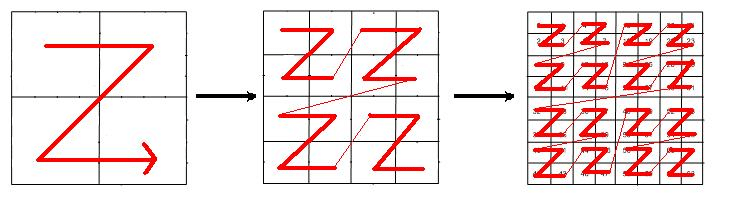
\includegraphics[width=.5\linewidth]{figs/Morton.jpg}
	\caption{Morton's order\citep{salem2016comparative}}
	\label{fig:morton}
\end{figure}
\end{frame}

\begin{frame}{Cholesky Factorization}
\footnotesize
With various $n$, three Cholesky methods are applied and results are below table \ref{tab:table1}. In low rank approximation at algorithm \ref{alg:hchol}, rank is about $n^{1/4}$.
\begin{table}[h]
	\centering
	% \resizebox{.6\textwidth}{!}{%
	{
		\begin{tabular}{@{}ccccc@{}}
			\toprule
			n & 256 & 1024 & 4096 & 16384 \\ \midrule
			chol & 0.001s & 0.0097s & 0.414s & 156.3s \\
			dpotrf & 0.0007s & 0.0132s & 0.431s & 154.1s \\
			hierarchical cholesky & 0.153s & 0.076s & 0.916s & 37.3s \\
			Error of hierarchical cholesky & 1.06e-7 & 9.97e-7 & 1.11e-3 & 1.87e-3 \\  \bottomrule
		\end{tabular}%
	}
	\caption{Excution times for Cholesky factorization}
	\label{tab:table1}
\end{table}
\begin{itemize}
	\item Hierarchical cholesky decomposition is more efficient than other classical cholesky method with large dimension.
	\item Hierarchical cholesky decomposition provides $\boldsymbol{\Sigma}\approx L_HL_H^T$. Its relative error is defined as $\frac{\lVert\boldsymbol{\Sigma}-L_HL_H^T\rVert_2}{\lVert\boldsymbol{\Sigma}\rVert_2}$
	\item Table \ref{tab:table1} ensures accuracy of hierarchical cholesky decomposition proposed by \citet{hackbusch2015hierarchical}.
\end{itemize}
\end{frame}

\begin{frame}{Multivariate Normal Probabilities} 
\end{frame}
	
	
	
\begin{frame}{d-dimensional Conditioning Algorithm without/with Reordering}
\footnotesize
	
\begin{theorem}\label{thm:haar}\citet{stewart1980efficient}
	Let the independent vectors $x_1,\cdots,x_{n}$ be distributed $N(0,\sigma^2 \mathbf{I})$. For $j=1,2,\cdots,n-1$, let $\mathbf{\bar{H}}_{x_j}$ be the Householder transformation that reduces $x_j$ to $r_{jj}e_1$, where $r_{ij}$ is obtained in QR decomposition of $[x_1,\cdots,x_n]$ Let $\mathbf{H}_j=diag(\mathbf{I}_{j-1},\bar{\mathbf{H}}_j)$. Let $\mathbf{D}=diag(sign(r_{11}), \cdots, sign(r_{nn}))$. Then the product $\mathbf{Q}=\mathbf{DH_1\cdots H_{n-1}}$ follows Haar Distribution.
\end{theorem}

\begin{itemize}
	\item 250 MVN problems with various values of $m$ and $d$
	\item $\boldsymbol{\Sigma}=\mathbf{Q}\mathbf{J}\mathbf{Q}^T$ is simulated with $\mathbf{Q}\sim{Haar distribution}$ and $J=diag(j_i)$ where $j_1,\cdots,j_m\sim U(0,1)$
	\item Integration limits $a_i=-\infty$ and $b_i\sim(U,m)$ for $i=1\cdots,m$
	\item Estimated value is compared with approximated value obtained via quasi monte carlo method with a sample size of $10^4$, which ensures error below $10^{-4}$
\end{itemize}


\end{frame}
	
\begin{frame}{d-dimensional Conditioning Algorithm without/with Reordering}
\tiny

\begin{table}[h]
	\centering
	% \resizebox{.6\textwidth}{!}{%
	{
		\begin{tabular}{@{}cccccc@{}}
			\toprule
			$(m, d)$ & 1 & 2 & 4 & 8 & 16 \\ \midrule
			\multicolumn{6}{l}{Without univariate reordering} \\ \midrule
			\multirow{2}{*}{16} & 3.7\% & 3.5\% & 3.6\% & 3.8\% & 2.9\% \\
			& 0.029ms & 0.201ms & 0.431ms & 0.676ms & 1.372ms \\
			\multirow{2}{*}{32} & 2.4\% & 2.9\% & 2.9\% & 3.3\% & 2.7\% \\
			& 0.001ms & 0.390ms & 0.833ms & 1.283ms & 2.545ms \\
			\multirow{2}{*}{64} & 1.9\% & 2.1\% & 2.1\% & 1.8\% & 1.9\% \\
			& 0.004ms & 0.762ms & 1.686ms & 2.545ms & 5.004ms \\
			\multirow{2}{*}{128} & 1.3\% & 1.5\% & 1.3\% & 1.2\% & 1.4\% \\
			& 0.024ms & 1.505ms & 3.333ms & 5.146ms & 10.548ms \\ \midrule
			\multicolumn{6}{l}{With univariate reordering} \\ \midrule
			\multirow{2}{*}{16} & 3.3\% & 3.1\% & 3.3\% & 3.6\% & 2.7\% \\
			& 0.007ms & 0.203ms & 0.439ms & 0.680ms & 1.363ms \\
			\multirow{2}{*}{32} & 2.3\% & 2.6\% & 2.6\% & 3.2\% & 2.6\% \\
			& 0.004ms & 0.393ms & 0.841ms & 1.289ms & 2.544ms \\
			\multirow{2}{*}{64} & 2.0\% & 2.1\% & 2.1\% & 1.9\% & 1.9\% \\
			& 0.014ms & 0.773ms & 1.695ms & 2.552ms & 5.022ms \\
			\multirow{2}{*}{128} & 1.2\% & 1.5\% & 1.4\% & 1.2\% & 1.4\% \\
			& 0.097ms & 1.593ms & 3.462ms & 5.268ms & 10.7861ms \\ \bottomrule
		\end{tabular}%
	}
	\caption{Errors and execution times of the d-dimensional conditioning method}
	\label{tab:table2}
\end{table}
\footnotesize
Estimation error tended to decrease as $d$ increases with each $m$ since lager $d$ implers less discarded correlation information. Spent time grows to a linear fashion with m while it grows exponentially with $d$.
\end{frame}